\documentclass[letter, 12pt]{article}

\usepackage[margin=0.5in]{geometry}

%equation spacing
\usepackage{xpatch}
\xapptocmd\normalsize{%
 \abovedisplayskip=0pt plus 0pt minus 0pt
 \abovedisplayshortskip=0pt plus 0pt
 \belowdisplayskip=0pt plus 0pt minus 0pt
 \belowdisplayshortskip=0pt plus 0pt minus 0pt
}{}{}

% \usepackage{blindtext}
\usepackage{amssymb,amsfonts,amsmath}

%%%%%%%%%%%%%%%%%%%%%%%%%%%%%%
%% OPTIONAL MACRO FILES
%% Insert self-defined macros here.
%% \newcommand definitions are recommended; \def definitions are supported

\usepackage[pdftex]{graphicx}
\usepackage{amsthm}
\usepackage{textcomp}
\usepackage{latexsym}
\usepackage{enumerate}
\usepackage{natbib}

\newtheorem{thm}{Theorem}[section]
\newtheorem{cor}[thm]{Corollary}
\newtheorem{ex}[thm]{Example}
\newtheorem{conj}[thm]{Conjecture}
\newtheorem{prob}[thm]{Problem}
\newtheorem{lem}[thm]{Lemma}
\newtheorem{prop}[thm]{Proposition}
\theoremstyle{definition}
\newtheorem{defn}[thm]{Definition}
\theoremstyle{remark}
\newtheorem{rem}[thm]{Remark}
%\numberwithin{equation}{section}

\newcommand{\set}[1]{\lbrace #1 \rbrace}
\newcommand{\setc}[2]{\lbrace #1 \mid #2 \rbrace}
\newcommand{\vv}[1]{{\mathbf{#1}}}
\newcommand{\dd}{{\mathrm{d}}}
\newcommand{\pd}[2]{\frac{\partial #1}{\partial #2}}
\newcommand{\pdn}[3]{\frac{\partial^#1 #2}{\partial #3^#1}}
\newcommand{\od}[2]{\frac{\dd #1}{\dd #2}}
\newcommand{\odn}[3]{\frac{\dd^#1 #2}{\dd #3^#1}}
\newcommand{\avg}[1]{\left< #1 \right>}

%--- operators
\DeclareMathOperator{\trop}{trop}
\DeclareMathOperator{\adj}{adj}
\DeclareMathOperator{\tr}{tr}
\DeclareMathOperator*{\argmax}{argmax}
\DeclareMathOperator{\Var}{Var}

\newcommand{\mb}{\mathbf}
\newcommand{\argmin}{\operatornamewithlimits{argmin}}
\newcommand{\doublebar}{\bigl|\!\bigr|}

% Default fixed font does not support bold face
\DeclareFixedFont{\ttb}{T1}{txtt}{bx}{n}{12} % for bold
\DeclareFixedFont{\ttm}{T1}{txtt}{m}{n}{12}  % for normal

% Custom colors
\usepackage{color}
\definecolor{deepblue}{rgb}{0,0,0.5}
\definecolor{deepred}{rgb}{0.6,0,0}
\definecolor{deepgreen}{rgb}{0,0.5,0}

\usepackage{listings}

% Python style for highlighting
\newcommand\pythonstyle{\lstset{
language=Python,
basicstyle=\ttm,
otherkeywords={self},             % Add keywords here
keywordstyle=\ttb\color{deepblue},
emph={},          % Custom highlighting
emphstyle=\ttb\color{deepred},    % Custom highlighting style
stringstyle=\color{deepgreen},
%frame= tb,                         % Any extra options here
showstringspaces=false            % 
}}


% Python environment
\lstnewenvironment{python}[1][]
{
\pythonstyle
\lstset{#1}
}
{}

% Python for external files
\newcommand\pythonexternal[2][]{{
\pythonstyle
\lstinputlisting[#1]{#2}}}

% Python for inline
\newcommand\pythoninline[1]{{\pythonstyle\lstinline!#1!}}


\newcommand{\commentfe}[1]{{\color{red}FE: #1}}

\begin{document}

\title{Starter Manual for \texttt{hdnet} in Python}
\author{\normalsize Christopher Hillar, Redwood Center for Theoretical Neuroscience, Berkeley, CA, USA\\
\normalsize Felix Effenberger, Max-Planck-Institute for Mathematics in the Sciences, Leipzig, Germany
}
\date{}

\pagenumbering{gobble}


\maketitle

\textbf{Introduction}.  Here, we describe the basic functionality of the \texttt{hdnet} library in Python

\begin{center}
\texttt{https://github.com/team-hdnet/hdnet} \\
\end{center}

HDNET is a suite of powerful high-dimensional binary data modeling tools, with a specific emphasis on datasets coming from neuroscience.

For demonstration purposes we will start work with a synthetic data set  (later we will be working with spiking neural data). Spiking activity of 10 hypothetical cells is assumed to be given as iid. Poisson processes. Upon binning with a given bin width, this yields Bernoulli processes in discrete time. We create such Bernoulli data (as a proxy for real, binned spiking data) and then insert hypothetical correlations by means of a number of co-activations of different cell groups over time (also known as \textit{cell assemblies}).

The following script is contained in the file ``my\_first\_script.py".  We first import the necessary modules into our Python session (we recommend using ipython in pylab mode, i.e. running \texttt{ipython --pylab} and to run text copied to the clipboard from this tutorial using the magic command \texttt{\%paste}).

\begin{python}
import numpy as np
import matplotlib.pyplot as plt
from hdnet.spikes import Spikes
from hdnet.spikes_model import SpikeModel, BernoulliHomogeneous, \
	DichotomizedGaussian
\end{python}

We create two trials of $200$ time bins of spikes from $10$ neurons.

\begin{python}
spikes = (np.random.random((2, 10, 200)) < .05).astype(int)
spikes[0, [1, 5], ::5] = 1 # insert correlations
spikes[1, [2, 3, 6], ::11] = 1  # insert correlations
spikes = Spikes(spikes=spikes)
\end{python}

We can now plot a raster of the trials and covariances:

\begin{python}
plt.figure()
plt.title('Raw spikes')}
plt.matshow(spikes.rasterize(), cmap='gray')} 

plt.figure()
plt.title('Raw spikes covariance')
plt.matshow(spikes.covariance().reshape((2 * 10, 10)), cmap='gray')}

plt.show()
\end{python}

Next, we would like to model this noisy binary data.   First, we try to model each trial with a separate i.i.d. Bernoulli random binary vector having the same neuron means as in each trial:

\begin{python}
spikes_model = BernoulliHomogeneous(spikes=spikes)
BH_sample_spikes = spikes_model.sample_from_model()

plt.figure()
plt.title('BernoulliHomogeneous sample')
plt.matshow(BH_sample_spikes.rasterize(), cmap='gray')

plt.figure()
plt.title('BernoulliHomogeneous covariance')
plt.matshow(BH_sample_spikes.covariance().reshape((2 * 10, 10)), cmap='gray')

plt.show()
\end{python}
 
\begin{figure}
\begin{center}
\textbf{a)}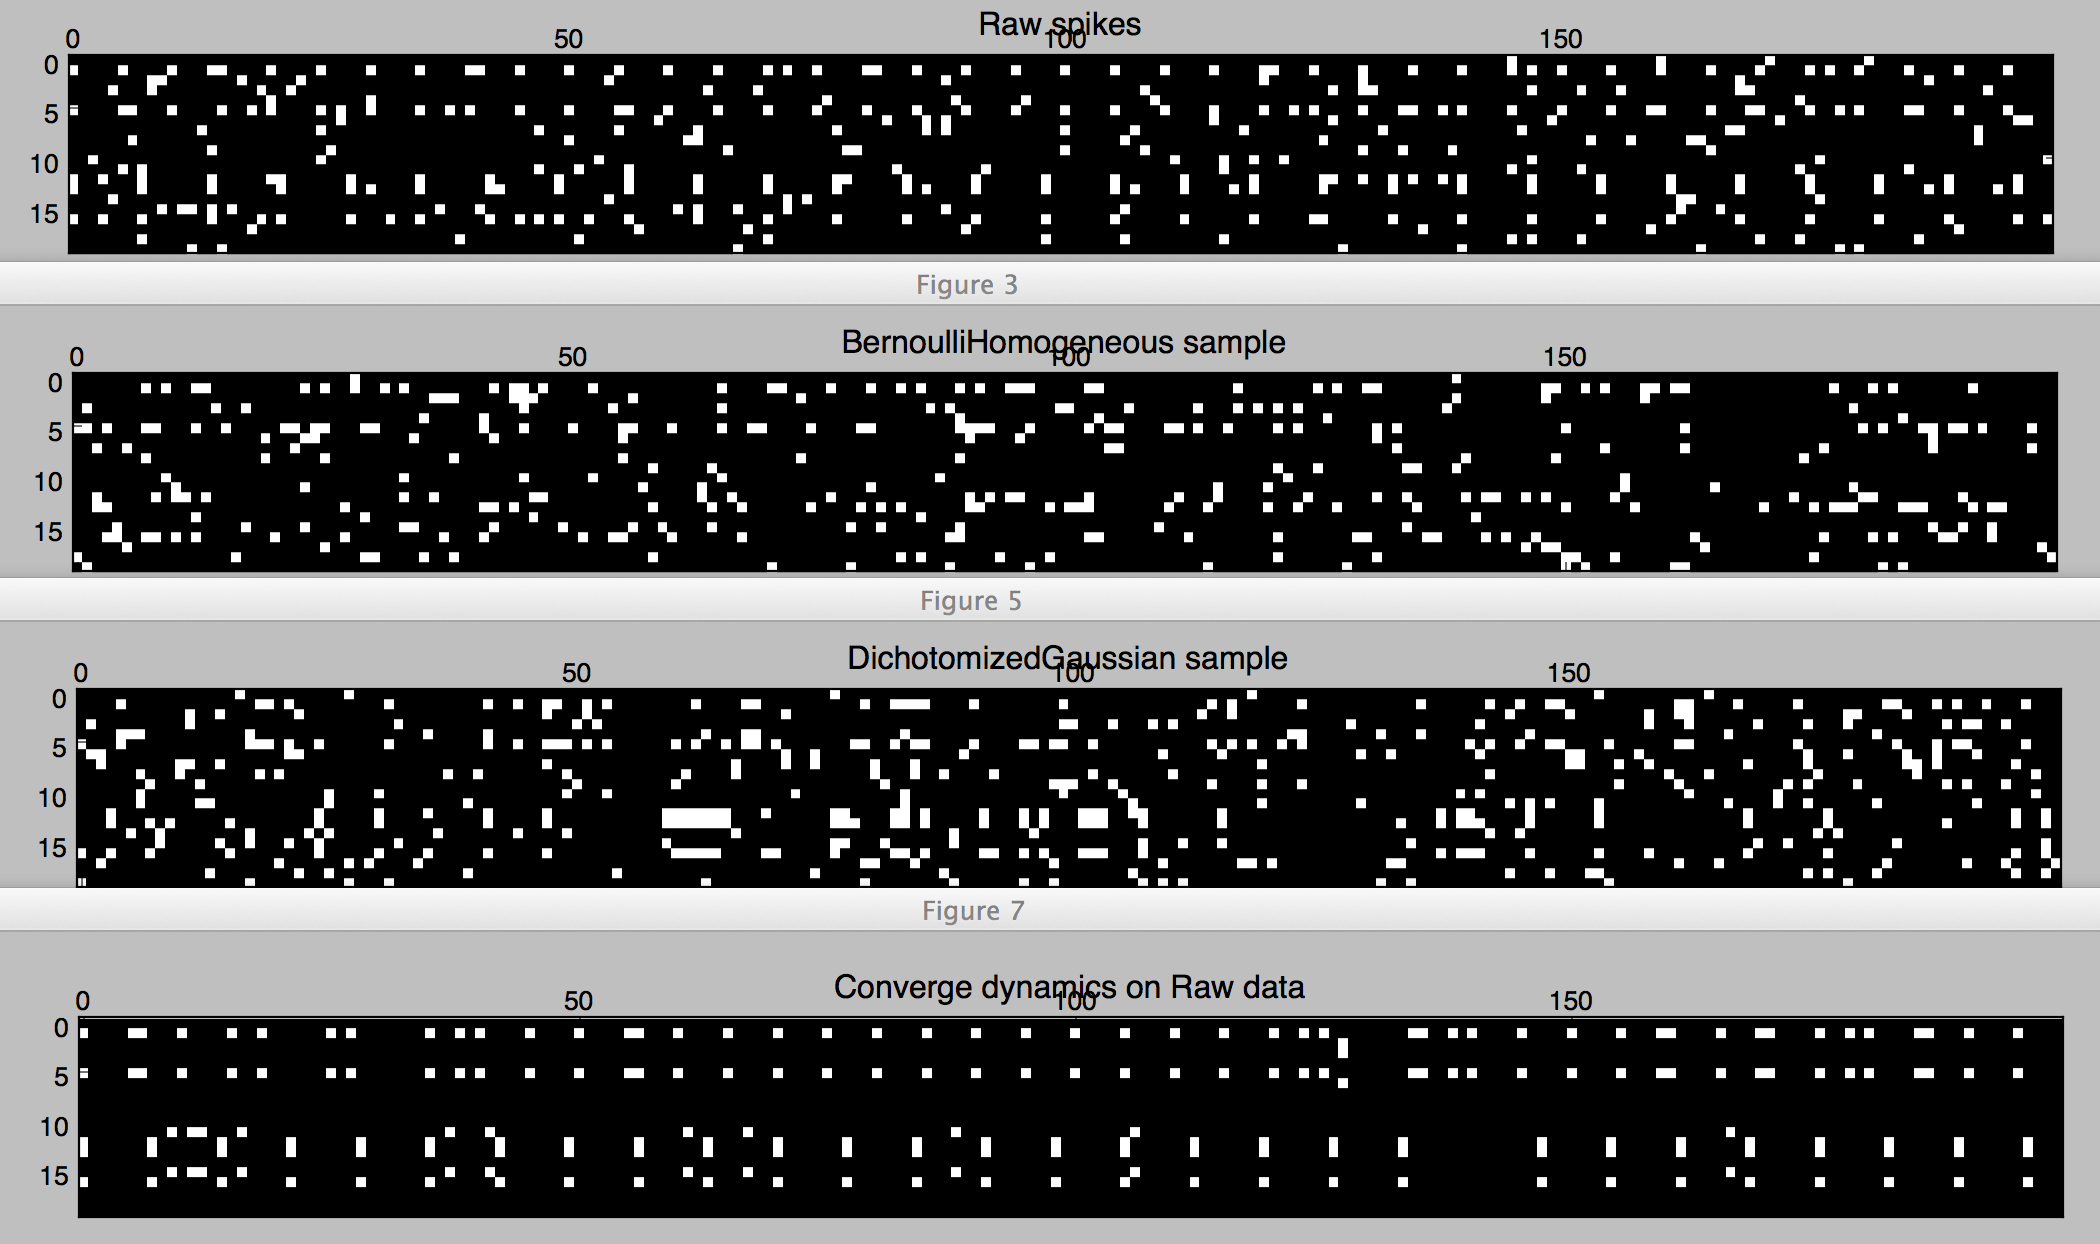
\includegraphics[width=.41\linewidth]{demo_fake_spikes.png} 
\textbf{b)}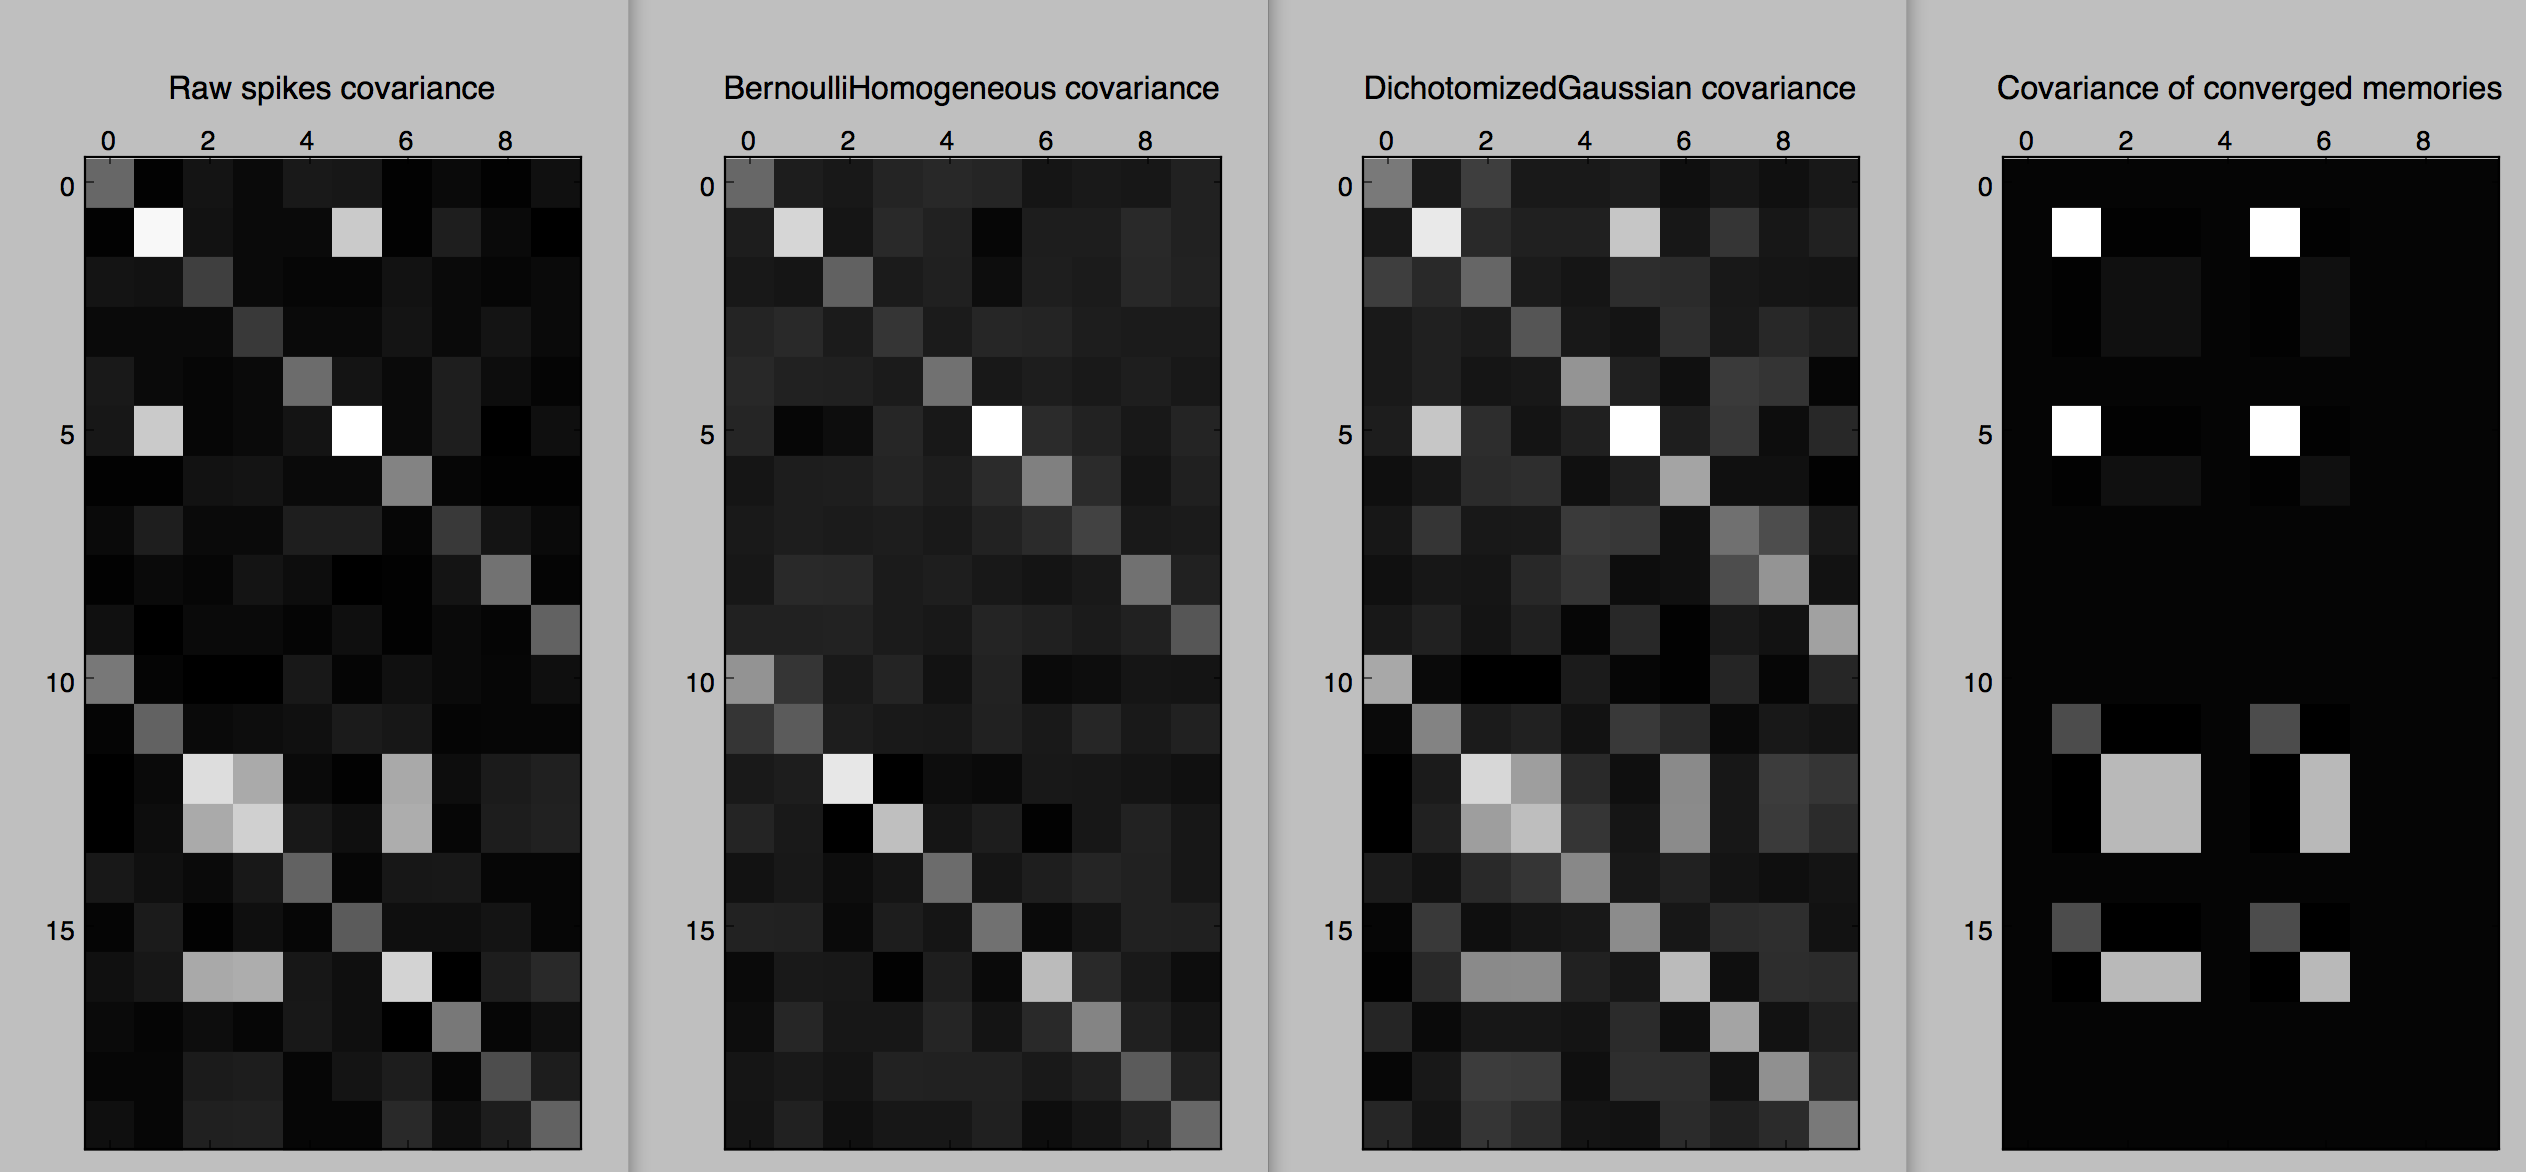
\includegraphics[width=.53\linewidth]{cov_demo.png} 
\caption{\textbf{Fake data example}. Two trials with 10 neurons.}
\label{fake_ex_fig}
\vspace{-.8cm}
\end{center}
\end{figure}

As we can see in Fig.~\ref{fake_ex_fig}, the samples from Bernoulli have the correct firing rates in each trial, but not the coordinated aspect (as can be seen in the covariance matrices for each trial, which are basically diagonal matrices).   A better model that keeps track of the correlations is the Dichotomized Gaussian \cite{bethge2008}: \\

\begin{python}
spikes_model = DichotomizedGaussian(spikes=spikes)
DG_sample_spikes = spikes_model.sample_from_model()

plt.figure()
plt.title('DichotomizedGaussian sample')
plt.matshow(DG_sample_spikes.rasterize(), cmap='gray')

plt.figure()
plt.matshow(DG_sample_spikes.covariance().reshape((2 * 10, 10)), cmap='gray')
plt.title('DichotomizedGaussian covariance')

plt.show()
\end{python}

Finally, we try and model the data with a Hopfield network trained using MPF \cite{HS-DK201} over all the trials:

\begin{python}
spikes_model = SpikeModel(spikes=spikes)
spikes_model.fit()  # note: this fits a single network to all trials
spikes_model.chomp()

converged_spikes = Spikes(spikes=spikes_model.hopfield_spikes)

plt.figure()
plt.title('Converge dynamics on Raw data')
plt.matshow(converged_spikes.rasterize(), cmap='gray')

plt.figure()
plt.title('Covariance of converged memories')
plt.matshow(converged_spikes.covariance().reshape((2 * 10, 10)), cmap='gray')

plt.show()
\end{python}

\textbf{More advanced features}.  One thing we would like to do is examine the structure of the memories:

\begin{python}
# plot memory label (its chronological appearance) as a function of time
plt.figure()
plt.scatter(range(len(spikes_model.memories.sequence)),
		1 + np.array(spikes_model.memories.sequence))
plt.xlabel('time bin')
plt.ylabel('Memory number (chronological order of appearance)')
plt.title('Converged memory label at each time bin')

# versus the raw data
plt.figure()
plt.scatter(range(len(spikes_model.empirical.sequence)),
		1 + np.array(spikes_model.empirical.sequence))
plt.ylabel('Raw pattern number (chronological order of appearance)')
plt.xlabel('time bin')
plt.title('Raw pattern label at each time bin')

plt.show()
\end{python}
 
Notice in Fig.~\ref{fake_ex_fig2} that the converged dynamics of the trained Hopfield network on the original data does reveal the 
hidden assemblies for the most part.

\begin{figure}[t!]
\begin{center}
\textbf{a)}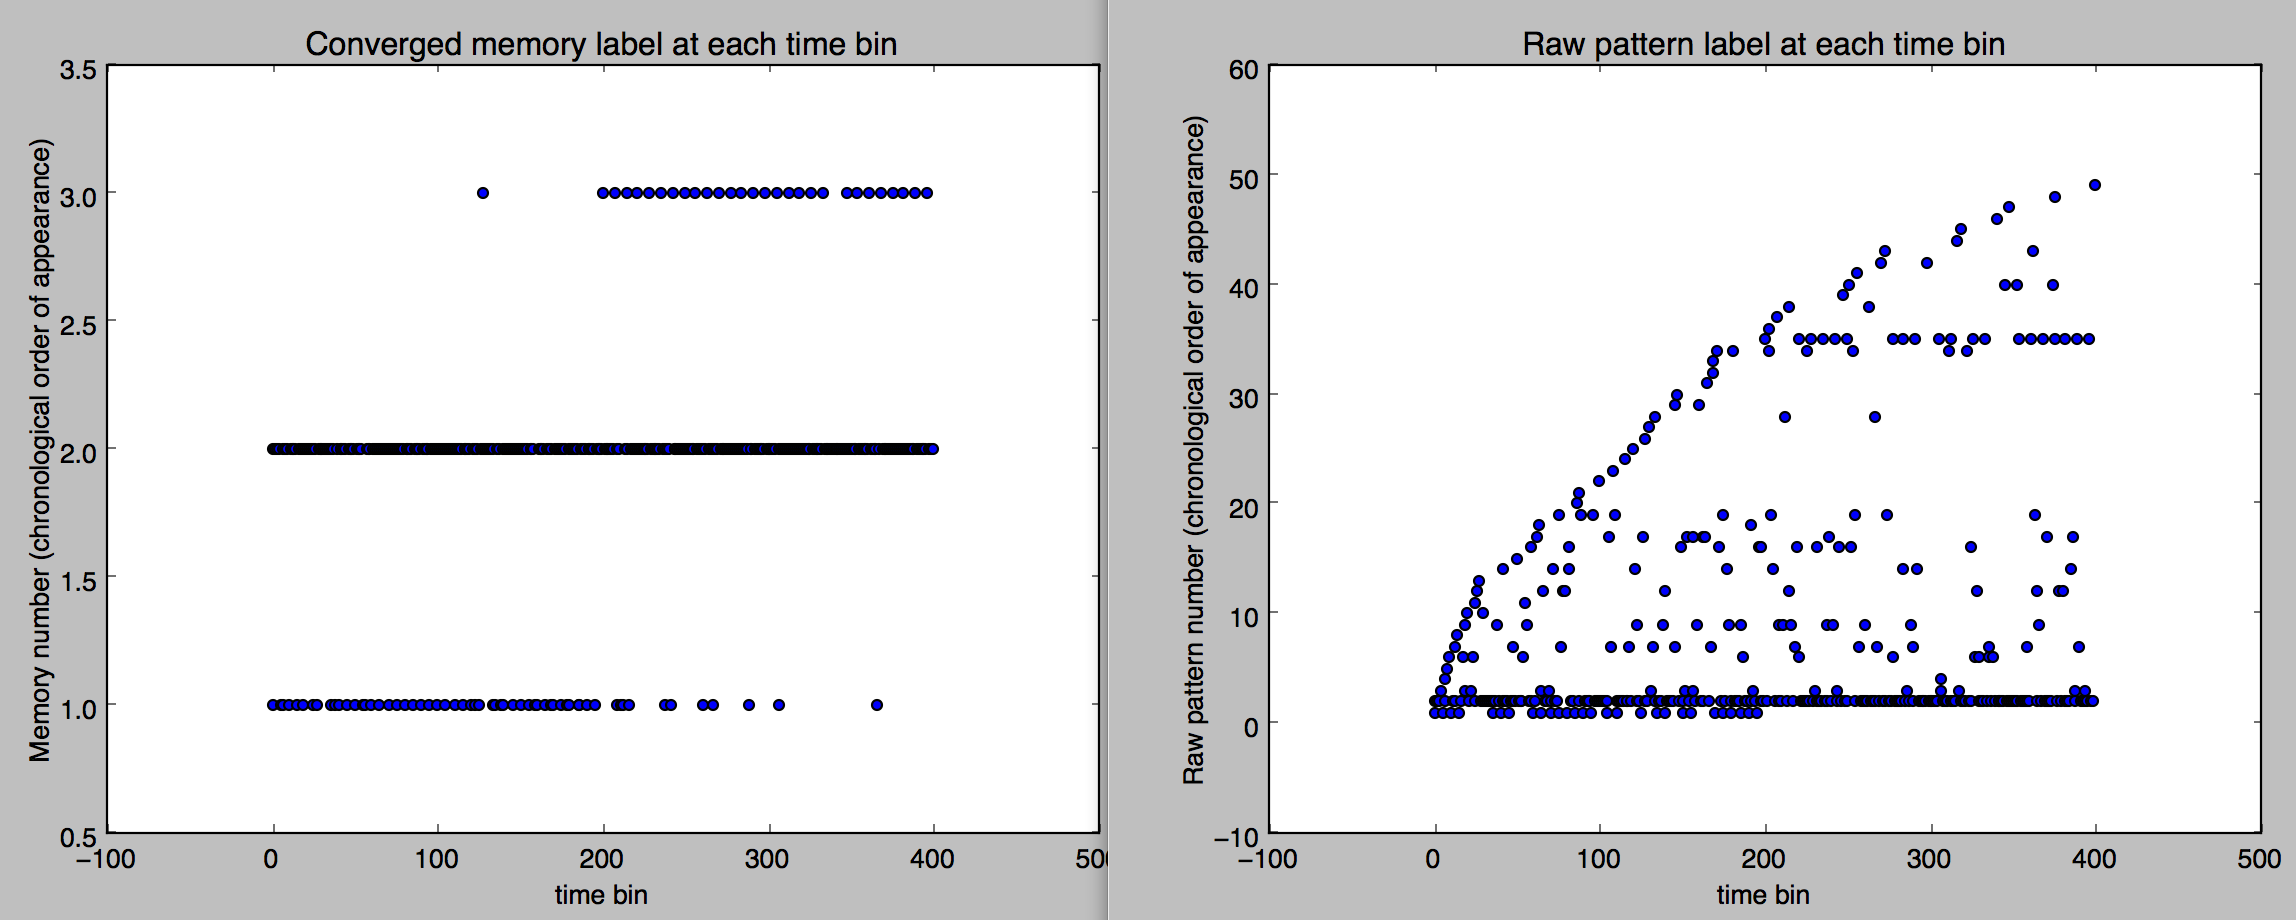
\includegraphics[width=.75\linewidth]{chron_order_patterns.png} 
%\textbf{b)}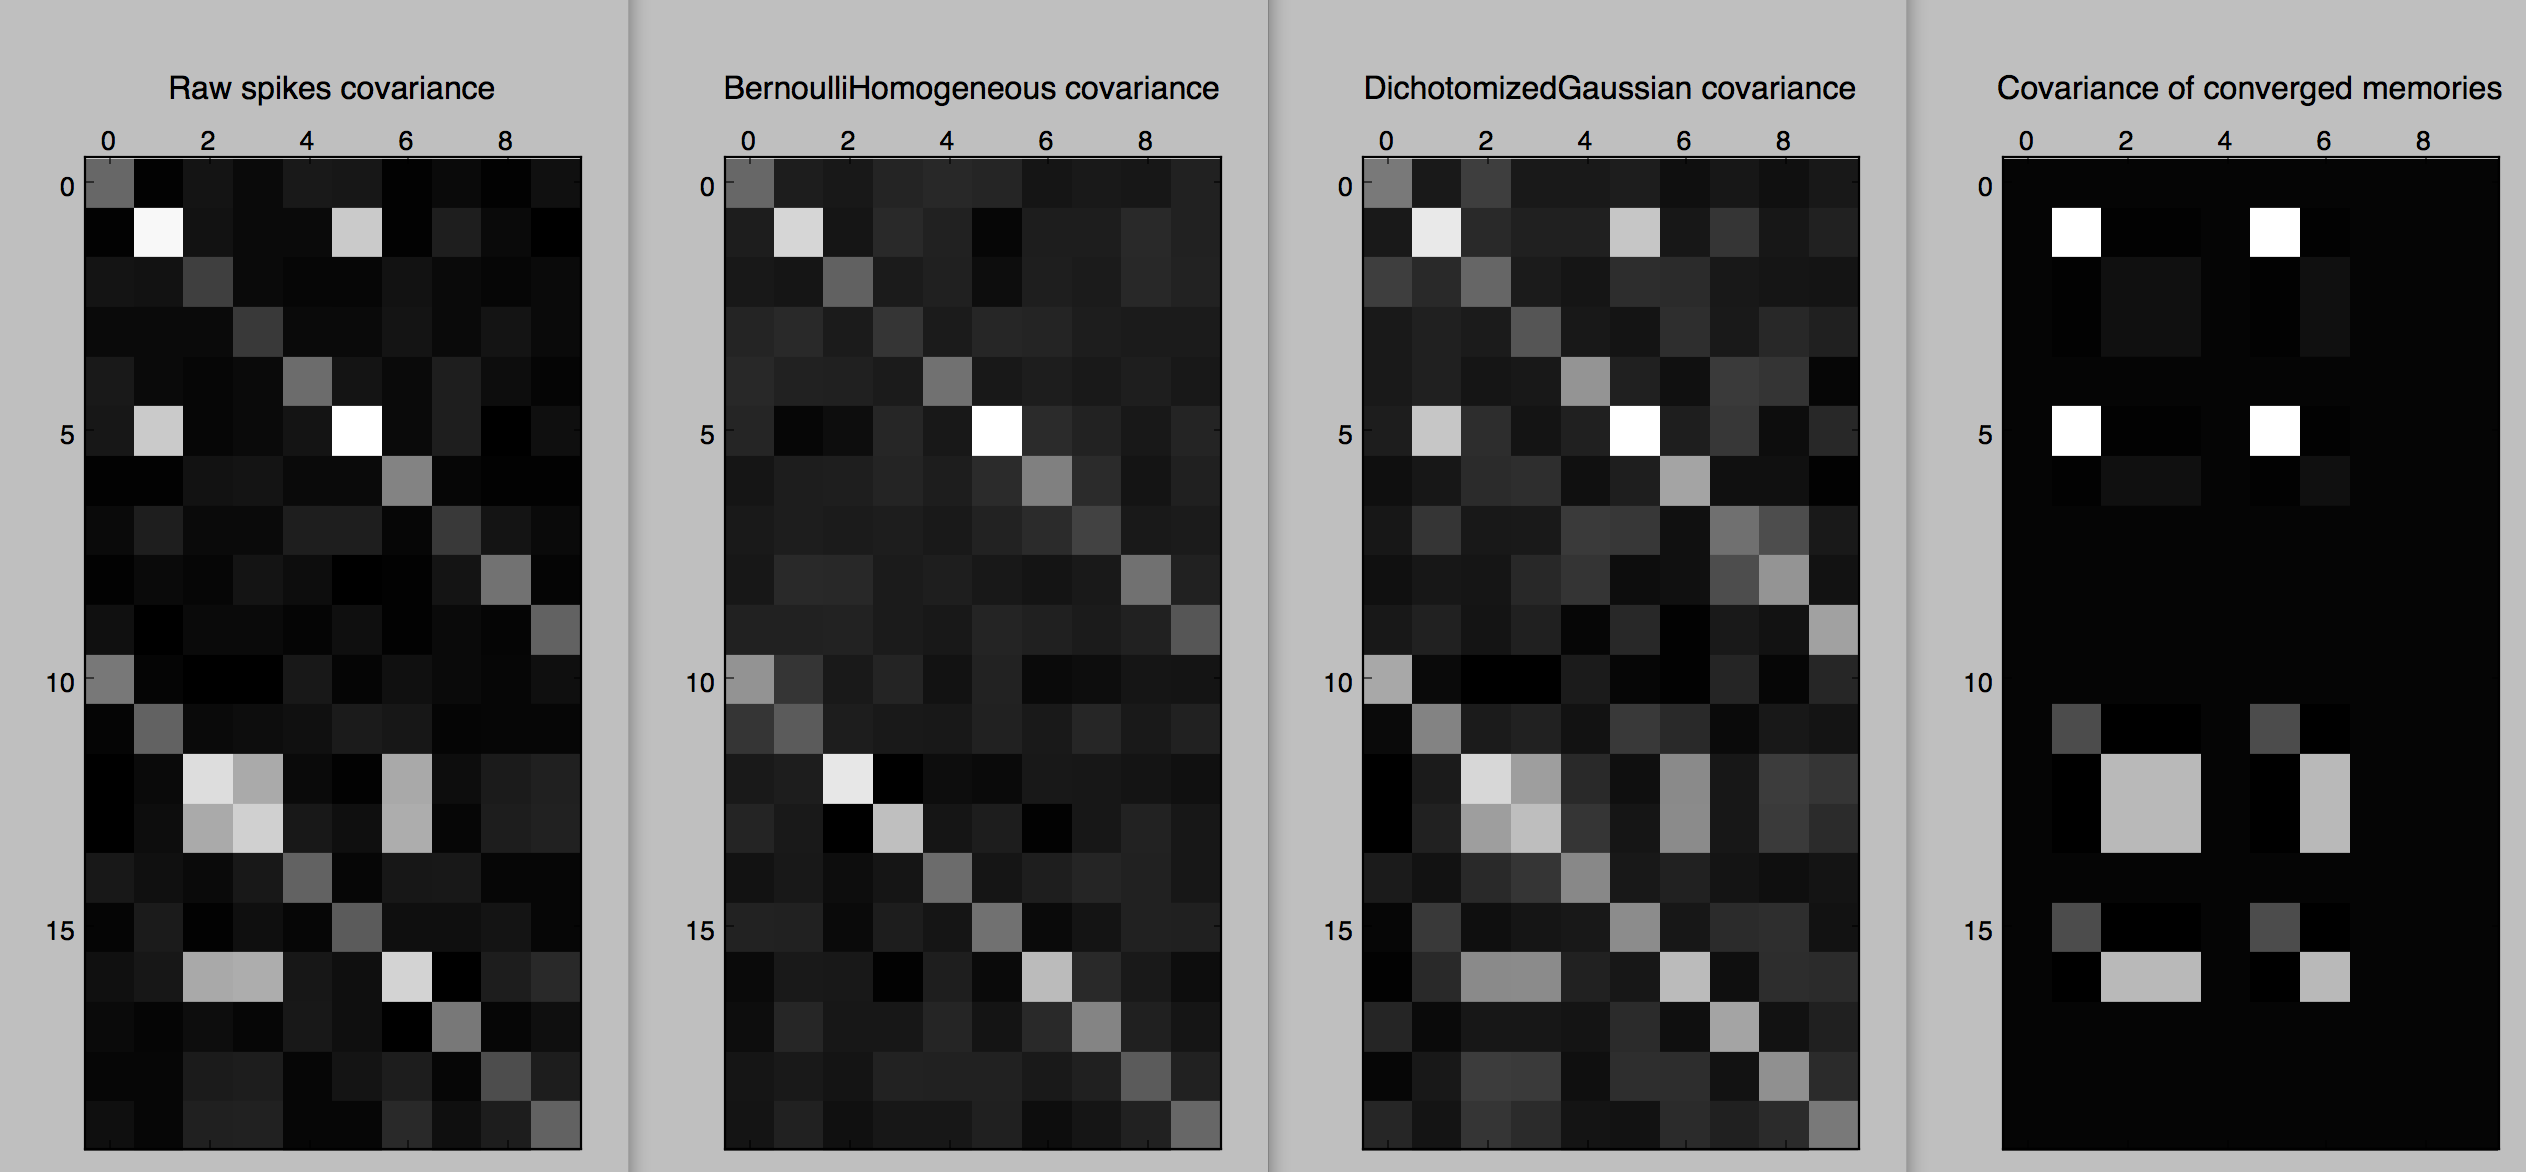
\includegraphics[width=.53\linewidth]{cov_demo.png} 
\textbf{b)}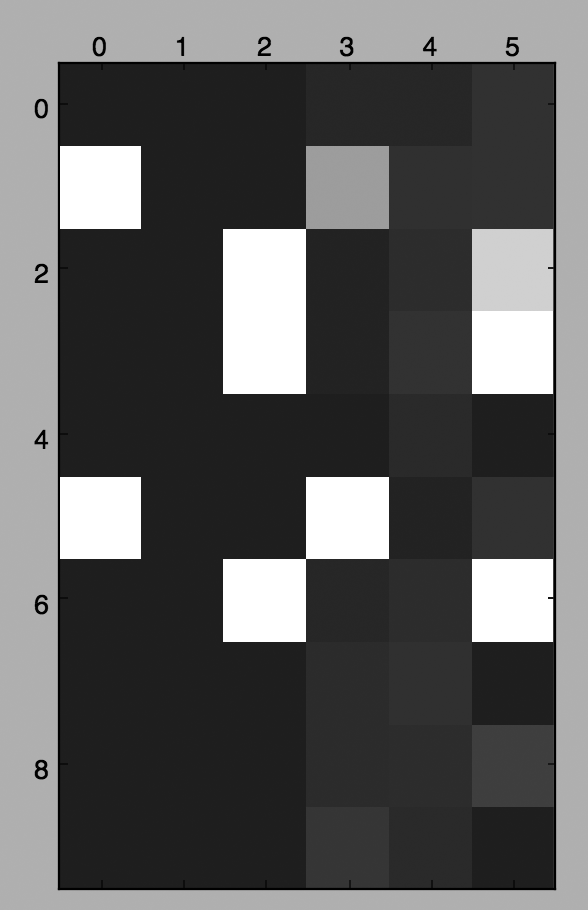
\includegraphics[width=.19\linewidth]{memories_stas.png} 
\caption{\textbf{Continuing fake data example}. \textbf{a)} Patterns (Converged at left, Raw on right) over time bins labeled on the $y$-axis by their first appearance in the dataset.  \textbf{b)}  Memories in network (left) and Memory Triggered Averages (at right).}
\label{fake_ex_fig2}
\vspace{-.8cm}
\end{center}
\end{figure}

Now that we know there are basically two assemblies, one showing up lots in the first trial and the other in the second, let's look at the
memories and their corresponding MTA's (\textit{memory triggered averages}).  The code below generates Fig.~\ref{fake_ex_fig2}\textbf{b}, which displays
a matrix whose first 3 columns are the memories in the network and whose next 3 columns are the average of Raw data patterns converging to the corresponding memory in the first 3 columns.

\begin{python}
# memories are ordered by their first appearance
bin_memories = spikes_model.memories.patterns
arr = np.zeros((spikes_model.original_spikes.N, 2 * len(bin_memories)))
for c, memory in enumerate(bin_memories):
	arr[:, c] = spikes_model.memories.fp_to_binary_matrix(c)

for c, memory in enumerate(bin_memories):
	arr[:, c + len(bin_memories)] = spikes_model.memories.mtas[memory] /
			spikes_model.memories.counts[memory]

print "Probabilities of each memory:"
print zip(bin_memories, spikes_model.memories.to_prob_vect())

# Probabilities of each memory:
# [('0100010000', 0.13), ('0000000000', 0.79249999999999998), /
# ('0011001000', 0.077499999999999999)]
\end{python}

Notice that the number of occurrences of the cell assembly with neuron 1 and 5 co-active is about double that of 2, 3, 6 co-active, consistent with our data insertions. \\


\textbf{Saving}.  One can save Learners and Memories.

\begin{python}
spikes_model.save('my_spikes_model')
loaded_spikes_model = SpikesModel.load('my_spikes_model')
\end{python}


\textbf{Stimuli}.   Continuing our main synthetic example, we now discuss how to incorporate stimuli into our analyses.   First, let's create a fake stimulus consisting of random normal $90 \times 100$ dimensional numpy arrays unless the fake stimulus is presented, in which case it is either a picture of Hobbes or Calvin (with some small noise added).

\begin{figure}[t!]
\begin{center}
\textbf{a)}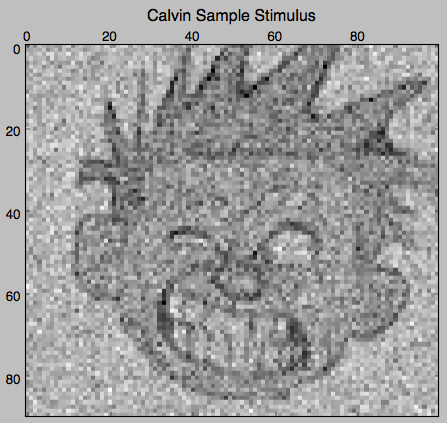
\includegraphics[width=.16\linewidth]{calvin_sample.png} 
\textbf{b)}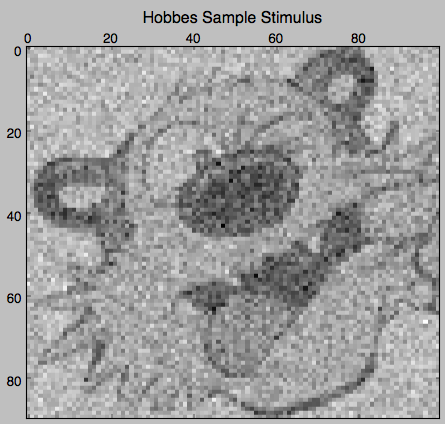
\includegraphics[width=.16\linewidth]{hobbes_sample.png} 
\textbf{c)}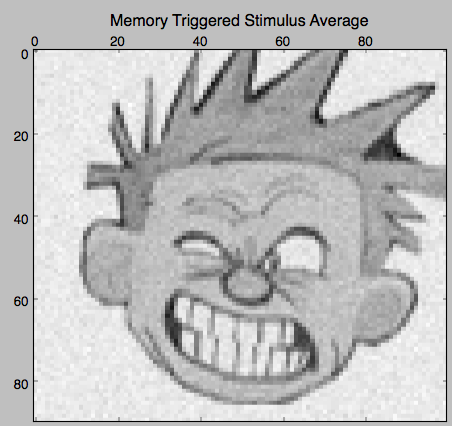
\includegraphics[width=.16\linewidth]{assembly1_memory_triggered_stimulus_avg.png} 
\textbf{d)}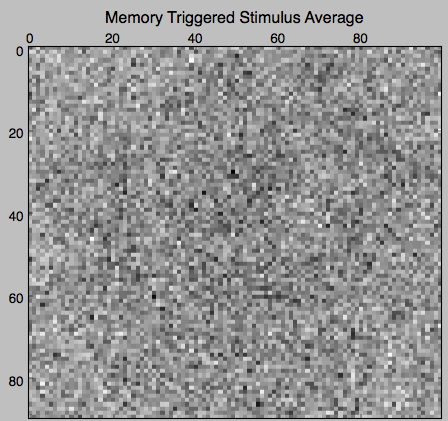
\includegraphics[width=.16\linewidth]{zero_memory_triggered_stimulus_avg.png}
\textbf{e)}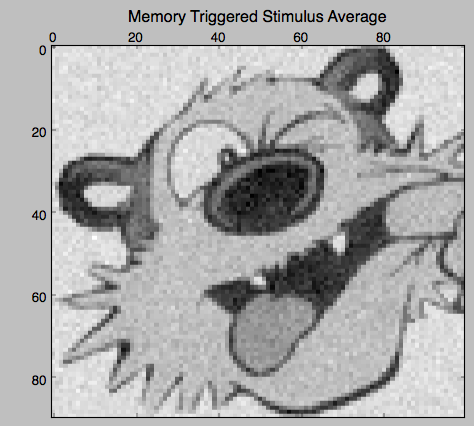
\includegraphics[width=.16\linewidth]{assembly2_memory_triggered_stimulus_avg.png}
\caption{\textbf{Continuing example with fake Stimuli}. \textbf{a, b)} Noisy stimuli: Calvin and Hobbes.  \textbf{c, d, e)}  Memory-triggered-stimulus averages of the Calvin, Empty, and Hobbes spike pattern in the fake data.}
\label{calvin_hobbes}
\vspace{-.8cm}
\end{center}
\end{figure}

\begin{python}
from hdnet.stimulus import Stimulus

calvin = np.load('data/calvin.npy')  # 90 by 100 numpy array
hobbes = np.load('data/hobbes.npy')

stimulus_arr = 20 * np.random.randn(2, 200, *calvin.shape)
stimulus_arr[0, ::5] = calvin + 50 * np.random.randn(200 / 5, *calvin.shape)
stimulus_arr[1, ::11] = hobbes + 50 * np.random.randn(200 / 11 + 1, /
						*hobbes.shape)

plt.matshow(stimulus_arr[0, 0], cmap='gray')
plt.title('Calvin Sample Stimulus')
plt.matshow(stimulus_arr[1, 0], cmap='gray')
plt.title('Hobbes Sample Stimulus')
\end{python}

Now, let's try and see what were the average stimuli for each fixed-point / memory.  We call such features \textit{memory triggered stimulus averages} (MTSA).



\begin{python}
stimulus = Stimulus(stimulus_arr=stimulus_arr)
avgs = spikes_model.memories.mem_triggered_stim_avgs(stimulus)

for stm_avg in avgs:
    plt.matshow(stm_avg, cmap='gray')
    plt.title('Memory Triggered Stimulus Average')
\end{python}


\textbf{Real data}.  Now, we try these methods out on some real data.  First, we download polytrode data recorded by Tim Blanche in the laboratory of Nicholas Swindale, University of British Columbia from the NSF-funded CRCNS Data Sharing website:

\begin{center}
\texttt{http://crcns.org/} \\
\end{center}

Let's examine the spontaneous spiking data from anesthetized cat visual cortex area 18 (around 5 minutes of spike-sorted polytrode data from 50 neurons).

\scriptsize
\setlength{\bibsep}{0pt plus 0.3ex}
\bibliographystyle{abbrv}
\bibliography{hdnet_manual} 

\end{document}
